\newpage
\section{Thuật toán phát sinh mê cung, các thuật toán tìm đường và gợi ý đường đi}

%--------------------------
%      Randomized DFS
%--------------------------

\subsection{Thuật toán phát sinh mê cung: Randomized DFS} 

\paragraph{}{Trong chương trình, chúng tôi sử dụng thuật toán \textbf{duyệt theo chiều sâu ngẫu nhiên} (randomized DFS) \cite{randomizeddfs} để sinh ra một mê cung. Thuật toán này sẽ sinh ra một mê cung có dạng cây. Tức là nếu coi mỗi ô trong ma trận là một đỉnh của đồ thị thì đồ thị này sẽ liên thông và không có chu trình. Điều này giúp đảm bảo từ một ô, ta có thể đi đến bất kỳ ô nào khác trong mê cung bằng một con đường duy nhất.}

\paragraph{}{Ban đầu, mê cung là một ma trận gồm có các ô trống, mỗi ô trống sẽ có 4 bức tường bao xung quanh.}

\begin{figure}[H]
    \centering
    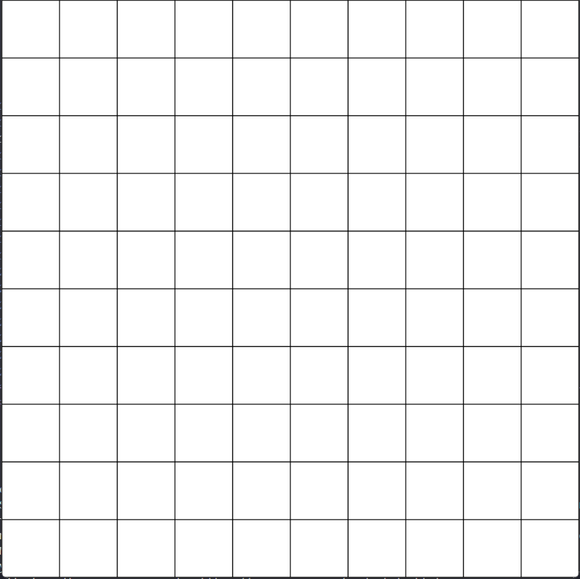
\includegraphics[width=0.3\linewidth]{img/init-maze-1.png}
    \caption{Ma trận các ô trống}
    \label{fig:init-maze-1}
\end{figure}

\paragraph{Thuật toán}
\paragraph{}{Thuật toán bắt đầu từ một ô bất kỳ trong mê cung, sau đó được thực hiện theo các bước:}

\paragraph{}{\textbf{Bước 1:} Gọi ô hiện tại đang được duyệt là ô $(x, y)$, ta thực hiện đánh dấu ô này là đã được duyệt qua.}
\paragraph{}{\textbf{Bước 2:} Lần lượt chọn các ô xung quanh chung cạnh với ô $(x, y)$ theo một thứ tự ngẫu nhiên. Tạm gọi ô đang được chọn là ô $(nx, ny)$.}
\paragraph{}{\textbf{Bước 3:} Nếu ô $(nx, ny)$ chưa được duyệt thì ta gọi đệ quy duyệt tới ô đó và xóa đi bức tường giữa ô $(x, y)$ và ô $(nx, ny)$. Ngược lại không làm gì cả.}


\paragraph{}{Sau khi thực hiện xong thuật toán ta được một mê cung thỏa mãn tính chất ở trên.}

\begin{figure}[H]
    \centering
    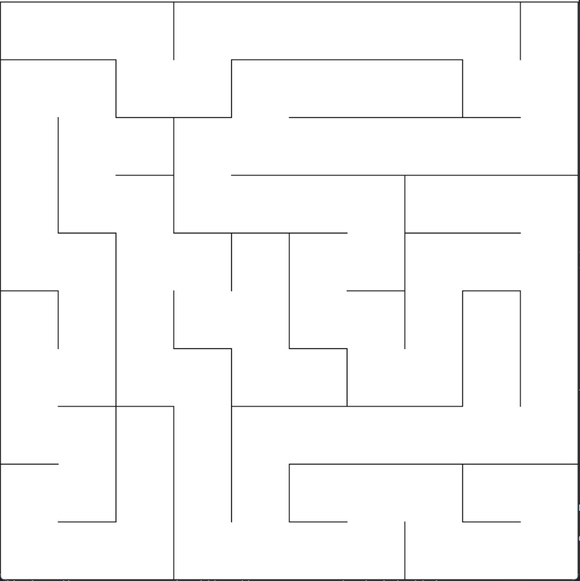
\includegraphics[width=0.3\linewidth]{img/init-maze-2.png}
    \caption{Mê cung được phát sinh sau khi thực hiện thuật toán}
    \label{fig:init-maze-2}
\end{figure}

\paragraph{Mã giả}{Thuật toán sinh mê cung randomized DFS}

\begin{algorithm}[H]
\caption{Randomized DFS}
\label{alg:rdfs}
\begin{algorithmic}
\Function {randomizedDFS}{\textit{x}, \textit{y}} 
\State // Đánh dấu đã duyệt ô (x, y)
\State $visited(x, y) \gets True$ 
\State
\State // Lấy danh sách các ô xung quanh (x, y) theo thứ tự ngẫu nhiên
\State $to\_visit \gets random\_shuffle(neighbor(x, y))$ 
\State

\For {$(nx, ny) \in to\_visit$}
\If {$visited(x, y) == False$}
\State loại bỏ bức tường nằm giữa hai ô (x, y) và (nx, ny)
\State randomizedDFS(nx, ny)
\EndIf
\EndFor
\EndFunction

\end{algorithmic}
\end{algorithm}

%--------------------------
%       BFS
%--------------------------

\subsection{Thuật toán tìm đường: BFS}
\paragraph{}{Thuật toán \textbf{duyệt đồ thị ưu tiên chiều rộng} \textit{(Breadth-first search - BFS)} là một trong những thuật toán tìm kiếm cơ bản và thiết yếu trên đồ thị. Ứng dụng của BFS có thể giúp ta giải quyết tốt một số bài toán trong thời gian và không gian \textbf{tối thiểu}. Đặc biệt là bài toán tìm kiếm đường đi ngắn nhất từ một đỉnh gốc tới tất cả các đỉnh khác. Trong bài toán tìm đường đi trong mê cung này, ta sẽ coi mỗi ô của mê cung là \textbf{1 đỉnh}, nếu từ 1 ô này có thể sang 1 ô khác thì sẽ có \textbf{1 cạnh} nối giữa 2 đỉnh này.}

\paragraph{Cơ chế hoạt động}
\paragraph{}{Từ một điểm xuất phát sẽ duyệt các điểm xung quanh có thể tới được, từ các điểm đã được duyệt đó sẽ thực hiện lại cơ chế trên để duyệt sang các điểm xung quanh khác, cứ như vậy cho đến khi duyệt tất cả các nhánh để tìm được nhánh có chứa đích đến thì dừng lại. Thứ tự ưu tiên của một đường đi thuật toán BFS là những đỉnh nào gần đỉnh xuất phát hơn sẽ được duyệt trước.}

\paragraph{Thuật toán}
\paragraph{}{Thuật toán sử dụng một hàng đợi (queue) để chứa các đỉnh. Các đỉnh này sau đó sẽ được duyệt theo quy tắc FIFO (first-in, first-out) của \textit{queue}. Tức là đỉnh nào vào \textit{queue} trước sẽ được duyệt trước.}

\paragraph{}{\textbf{Bước 1:} Khởi tạo}
\begin{itemize}
    \item Các đỉnh đều ở trạng thái chưa được đánh dấu, ngoại trừ đỉnh xuất phát \textbf{s} đã được đánh dấu.
    \item Một hàng đợi ban đầu chỉ chứa 1 phần tử là \textbf{s}.
\end{itemize}
\paragraph{}{\textbf{Bước 2:} Lặp lại các bước sau cho đến khi hàng đợi rỗng:}
\begin{itemize}
    \item Lấy đỉnh \textbf{u} ra khỏi hàng đợi.
    \item Xét tất cả những đỉnh \textbf{v} kề với \textbf{u} mà chưa được đánh dấu, với mỗi đỉnh \textbf{v} đó:
    \begin{itemize}
        \item Đánh dấu \textbf{v} đã thăm.
        \item Lưu lại vết đường đi từ \textbf{u} đến \textbf{v}.
        \item Đẩy \textbf{v} vào trong hàng đợi.
    \end{itemize}
\end{itemize}

\paragraph{Mã giả}{Thuật toán tìm đường BFS}

\begin{algorithm}[H]
\caption{BFS}
\label{alg:bfs}
\begin{algorithmic}
\Function {BFS}{\textit{startNode}, \textit{endNode}} // Đưa vào đỉnh bắt đầu và kết thúc

\State // Danh sách đỉnh cần duyệt sẽ được đưa vào một hàng đợi
\State $queue  \gets$ hàng\_đợi\_rỗng
\State đưa $startNode$ vào $queue$
\State
\State // Khởi tạo mảng 1 chiều visited đánh dấu những đỉnh đã thăm, giá trị khởi tạo là \textit{chưa thăm }
\State $visited[startNode] \gets$ đã thăm 
\State
\While{$queue$ không rỗng}
\State $currentNode \gets$ đỉnh tiếp theo trong queue
\If{$currentNode == endNode$}
\State \Return tồn tại đường đi từ đỉnh bắt đầu đến đỉnh kết thúc
\EndIf
\State Loại bỏ $currentNode$ khỏi $queue$
\For{$each neighbor \in$ các\_đỉnh\_kề$(currentNode)$} // duyệt các đỉnh kề đỉnh hiện tại
\If {$currentNode$ không thể tới được $neighbor$}
\State $continue$
\EndIf
\State $visited[neighbor] \gets$ đã thăm
\State đưa $neighbor$ vào $queue$
\EndFor

\Return không tồn tại đường đi từ đỉnh bắt đầu đến đỉnh kết thúc
\EndWhile
\EndFunction
\end{algorithmic}
\end{algorithm}

\paragraph{}{\textbf{Độ phức tạp thời gian:} Gọi $|V|$ là số lượng đỉnh và $|E|$ là số lượng cạnh của mê cung. Độ phức tạp thời gian của thuật toán này là $O(|V|+|E|)$.}

%--------------------------
%       A*
%--------------------------

\subsection{Thuật toán tìm đường: A*} 
\paragraph{}{A* \cite{astar} là giải thuật tìm kiếm trong đồ thị, tìm đường đi từ nút hiện tại đến đích sử dụng một hàm để ước lượng chi phí hay còn gọi là hàm heuristic. Từ trạng thái đường đi hiện tại, A* xây dựng tất cả các đường đi có thể, sử dụng hàm heuristic để đánh giá, tìm kiếm đường đi tối ưu và lưu giữ tập các lời giải trong một hàng đợi ưu tiên (priority queue). Thứ tự ưu tiên của một đường đi $x$ được quyết định bởi hàm $f(x) = g(x) + h(x)$.}
\paragraph{}{Trong đó:}
\begin{itemize}
    \item $g(x)$ là chi phí của đường đi từ nút xuất phát đến nút hiện tại.
    \item $h(x)$ là hàm đánh giá heuristic ước lượng chi phí từ nút hiện tại đến đích.
\end{itemize}
\paragraph{}{Hàm $f(x)$ có giá trị càng thấp thì độ ưu tiên càng cao. Có nghĩa là ta luôn ưu tiên duyệt các nút ở gần mục tiêu hơn. Nếu hàm heuristic $h$ có tính chất đơn điệu (hay nhất quán) tức thỏa mãn điều kiện $h(x) \leq d(x, y) + h(y)$ với mọi cạnh $x - y$ (ở đây $d(x, y)$ là độ dài cạnh $x - y$) thì thuật toán A* sẽ đảm bảo tìm ra một đường đi tối ưu.}
\paragraph{}{Vì bài toán tìm đường đi trong mê cung của ta là bài toán tìm đường đi trên cây có nghĩa là tồn tại một đường đi duy nhất từ đỉnh bắt đầu đến đỉnh kết thúc mà không đi qua một đỉnh quá hai lần nên ta không cần quan tâm đến tính đơn điệu của hàm heuristic. Điều này sẽ khiến thuật toán chạy nhanh hơn trong đa phần trường hợp. Trong chương trình, chúng tôi sử dụng hàm heuristic là bình phương khoảng cách euclid giữa điểm hiện tại và điểm kết thúc trong mê cung. Nói cách khác, nếu đỉnh hiện tại là ô $(x, y)$ và đỉnh kết thúc là ô $(endX, endY)$, ta có hàm heuristic:}

$$h(x, y) = (endX - x)^2 + (endY - y)^2$$

\paragraph{}{Khi di chuyển qua một ô thì độ dài đường đi tăng thêm 1 nên nếu đỉnh hiện tại là ô $(x, y)$ và đỉnh tiếp theo là ô $(u, v)$, ta có:}

$$g(u, v) = g(x, y) + 1$$
\paragraph{}{Vậy ta có \textbf{độ ưu tiên} cho ô $(u, v)$ nếu ô trước đó là ô $(x, y)$:
\begin{align*}
f(u, v) &= g(u, v) + h(u, v) \\
&= [g(x, y) + 1] + [(endX - u)^2 + (endY - v)^2]
\end{align*}}

\paragraph{}{\textbf{Mã giả} cho thuật toán A*:}


\begin{algorithm}[H]
\caption{A*}
\label{alg:rdfs}
\begin{algorithmic}
\Function {AStar}{\textit{startNode}, \textit{endNode}} // Đưa vào đỉnh bắt đầu và kết thúc
\State // Danh sách đỉnh cần duyệt sẽ được đưa vào một hàng đợi ưu tiên
\State $openSet \gets priority\_queue()$
\State // Chi phí của đường  từ điểm xuất phát đến điểm hiện tại
\State $g \gets$ \{giá trị các đỉnh: $\infty \forall$ đỉnh và 0 với đỉnh bắt đầu\}
\State // Tổng chi phí 
\State $f \gets$ \{giá trị các đỉnh: $\infty \forall$ đỉnh và $heuristic(startNode)$ với đỉnh bắt đầu\}
\State
\State Đưa cặp $startNode$ cùng chi phí $f(startNode)$ vào $openSet$
\While{$openSet$ không rỗng}
\State $currentNode \gets$ đỉnh trong openSet có tổng chi phí thấp nhất
\If{$currentNode == endNode$}
\State \Return tìm thấy đường đi
\EndIf
\State Loại bỏ $currentNode$ khỏi $openSet$
\State
\State // duyệt qua các đỉnh kề hợp lệ với đỉnh hiện tại
\For{$each$ $neighbor \in$ các\_đỉnh\_kề$(currentNode)$}
\State $newG \gets g(currentNode) + 1$
\State$ newF \gets newG + heuristic(currentNode)$
\If{$newG < g(neighbor)$}
\State $g(neighbor) \gets newG$
\State $f(neighbor) \gets newF$
\State đưa cặp $neighbor$ và $f(neighbor)$ vào $openSet$
\EndIf
\EndFor
\EndWhile
\Return thất bại, không tìm thấy đường đi
\EndFunction
\end{algorithmic}
\end{algorithm}

\paragraph{Độ phức tạp thời gian}
\paragraph{}{Độ phức tạp thời gian của thuật toán A* phụ thuộc vào đánh giá heuristic. Trong trường hợp tệ nhất, A* sẽ có độ phức tạp là $O(b^d)$ với $b$ là số cạnh trung bình của mỗi đỉnh và $d$ là số lượng nút trên đường đi tối ưu từ đỉnh bắt đầu đến đỉnh kết thúc. Mặc dù vậy, A* vẫn là một trong những thuật toán tìm kiếm đường đi tốt nhất trong hầu hết các trường hợp.}

\paragraph{Ví dụ minh hoạ}
\paragraph{}{Trong ví dụ này ta chỉ quan tâm đến cách thuật toán A* hoạt động trong một ma trận bất kỳ, không phải cách thuật toán hoạt động ở trong một mê cung. Giả sử ta có một ma trận kích thước $10 * 10$ như \hyperref[fig:astar_pic1]{hình 4} với ô màu đỏ là ô xuất phát và ô màu xanh là ô kết thúc. Các viền màu đen đậm hơn bên ngoài và viền màu đỏ ở trong là các bức tường. Ở đây, ta sẽ lập sẵn các bảng giá trị cho từng hàm để mô tả thuật toán tốt hơn.}

\begin{figure}[H]
    \centering
    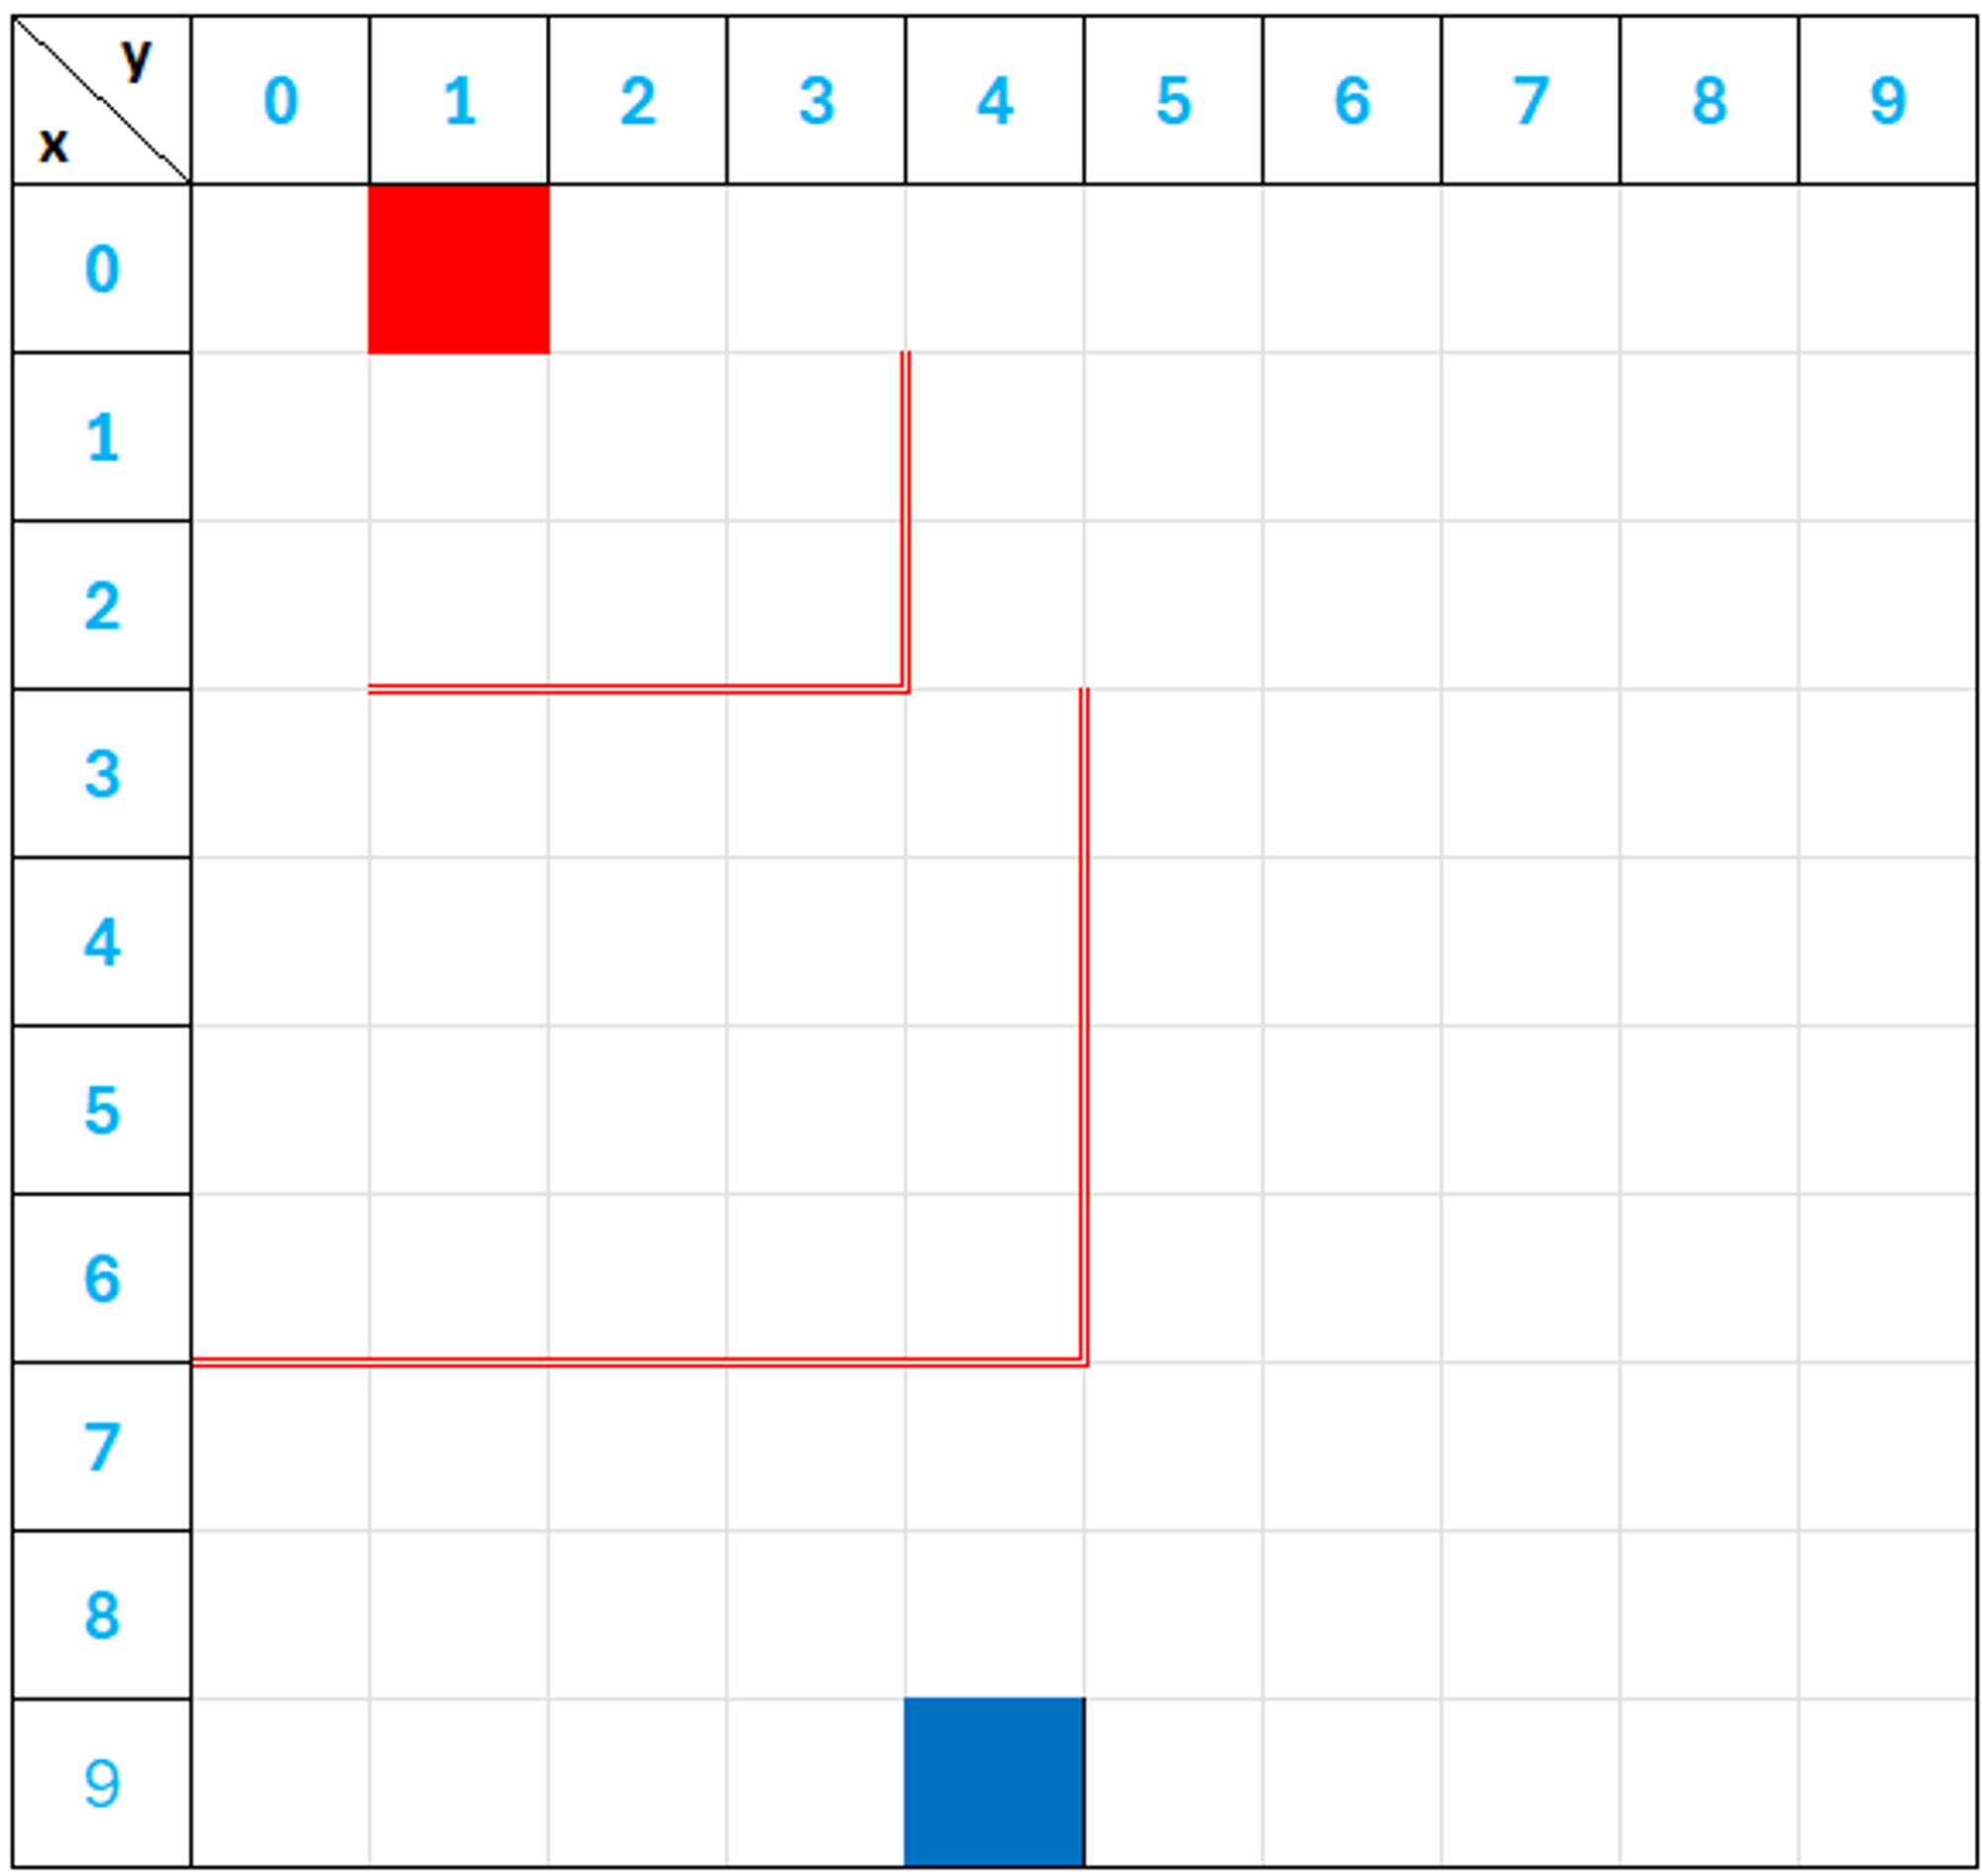
\includegraphics[width=0.5\linewidth]{img/astar_pic1.png}
    \caption{Ma trận giả định với điểm xuất phát, kết thúc và các bức tường}
    \label{fig:astar_pic1}
\end{figure}

\paragraph{}{Sử dụng công thức cho hàm $g(u, v)$ và $h(u, v)$ như đã nói ở trên, ta sẽ có được hai bảng giá trị cho hàm $g$ và $h$ như \hyperref[fig:astar_pic2]{hình 5}.}

\begin{figure}[H]
    \centering
    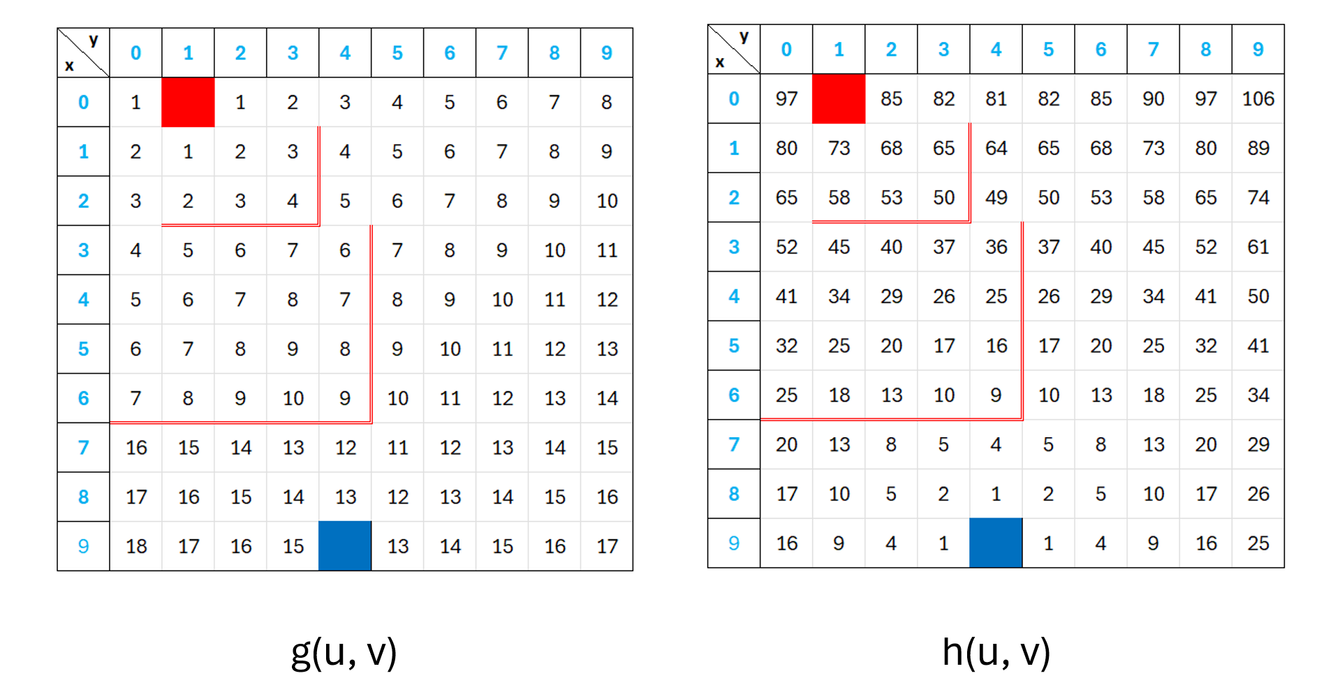
\includegraphics[width=1\linewidth]{img/astar_pic2.png}
    \caption{Bảng giá trị \textit{g} và \textit{h} trong ma trận}
    \label{fig:astar_pic2}
\end{figure}

Vì $f(u, v)$ = $g(u, v)$ + $h(u, v)$ nên ta sẽ có bảng cuối cùng như \hyperref[fig:astar_pic3]{hình 6}:

\begin{figure}[H]
    \centering
    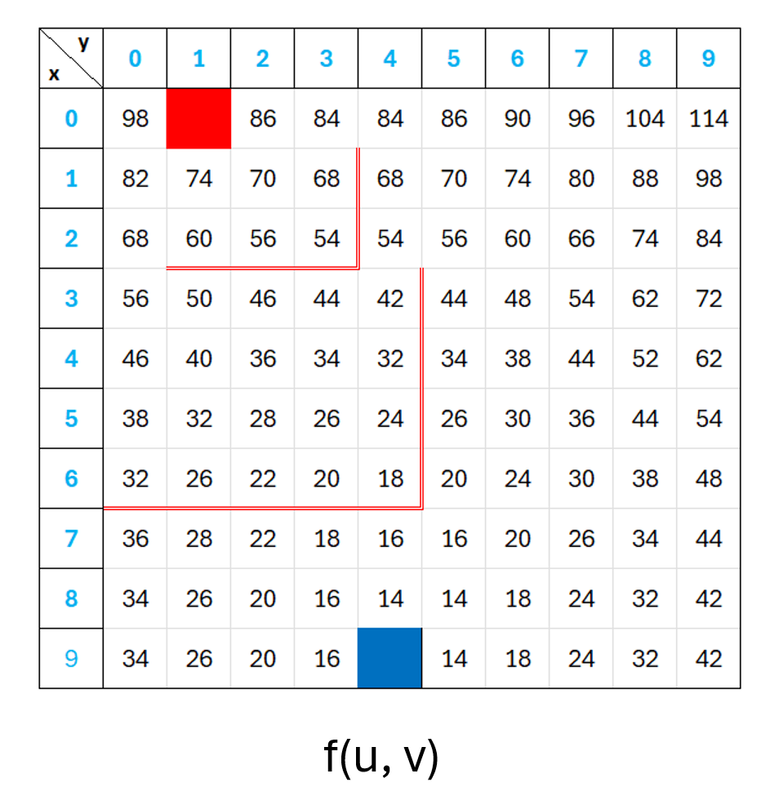
\includegraphics[width=0.5\linewidth]{img/astar_pic3.png}
    \caption{Bảng giá trị hàm \textit{f} trong ma trận}
    \label{fig:astar_pic3}
\end{figure}

Thuật toán khi bắt đầu chạy sẽ xuất phát ở ô màu đỏ là ô $(0, 1)$, duyệt qua các ô chung cạnh xung quanh để tìm một đường đi tới ô kết thúc. Thứ tự duyệt các ô sẽ dựa vào hàm $f(u, v)$ ta vừa tính được, ô có giá trị của hàm $f$ nhỏ hơn sẽ được ưu tiên duyệt trước. Ta có được sơ đồ đường đi của thuật toán như \hyperref[fig:astar_pic4]{hình 7}. Có thể thấy rằng, đường đi được tìm thấy không phải là đường đi ngắn nhất. Đó là bởi vì ta đã bỏ qua tính chất đơn điệu của hàm heuristic như đã nói ở trên.

\begin{figure}[H]
    \centering
    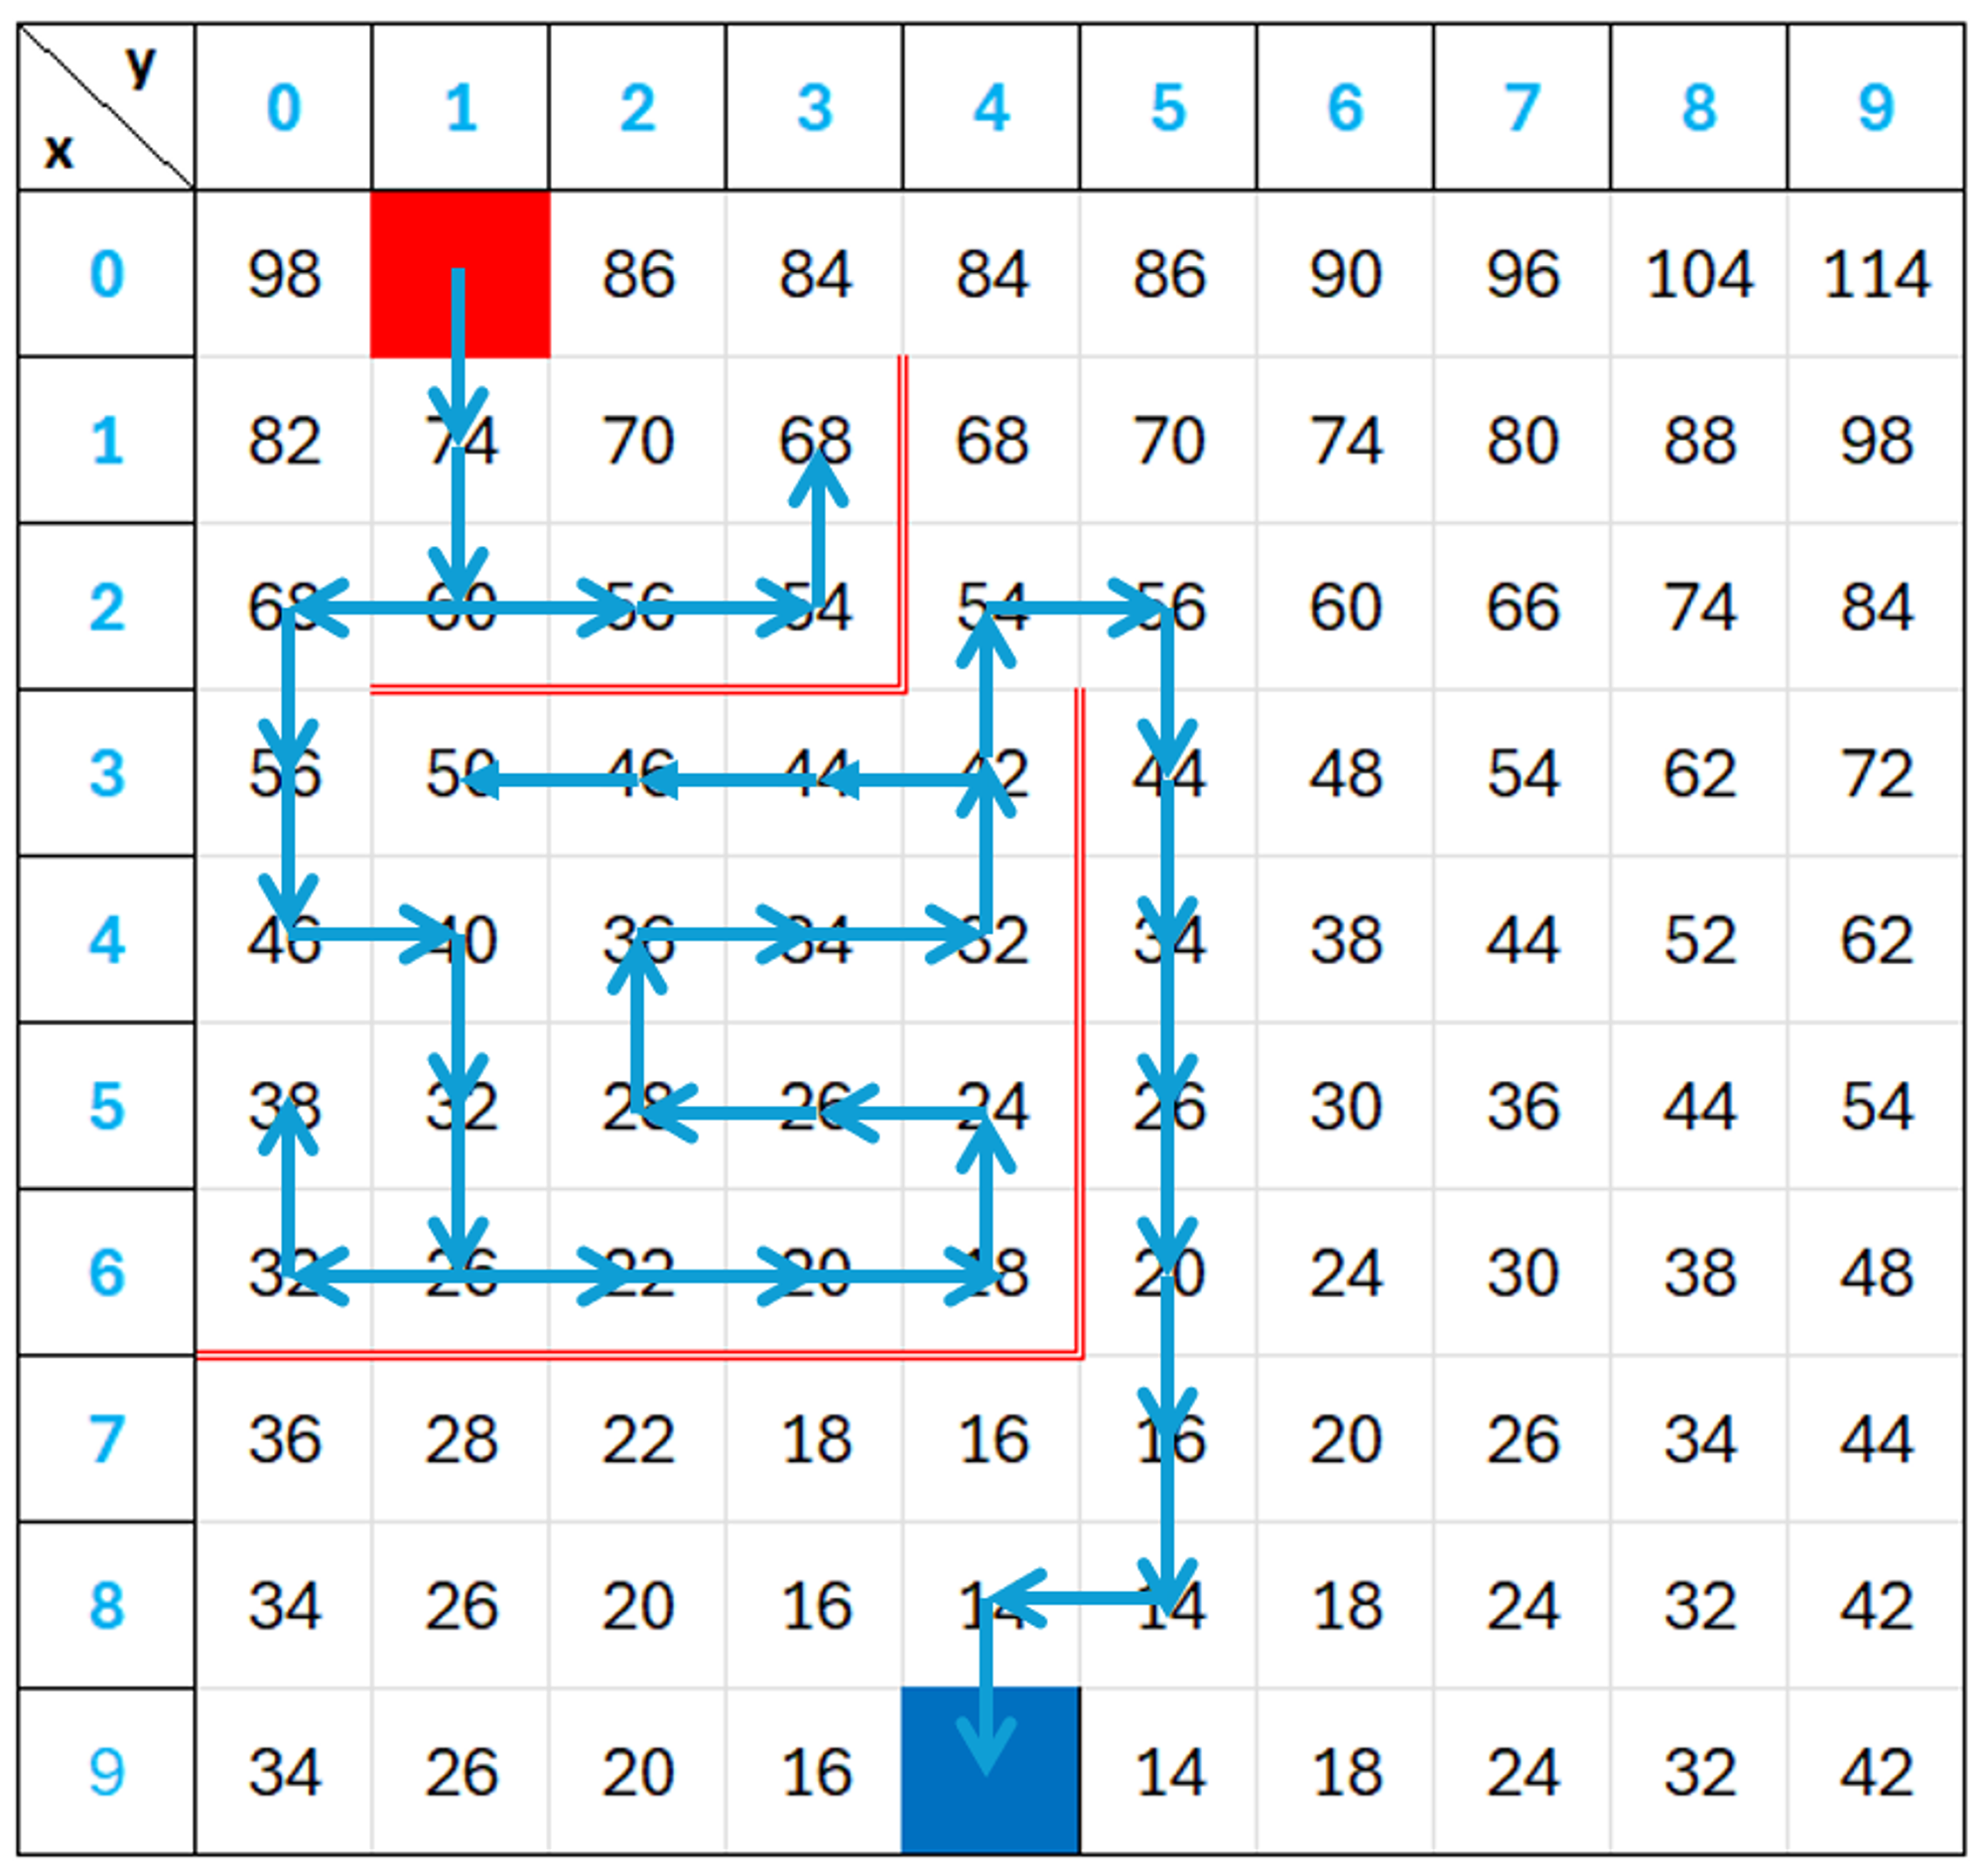
\includegraphics[width=0.5\linewidth]{img/astar_pic4.png}
    \caption{Sơ đồ đường đi thuật toán A*}
    \label{fig:astar_pic4}
\end{figure}

%--------------------------
%      So sanh thuat toan
%--------------------------

\subsection{So sánh thuật toán tìm đường BFS và A*}

\paragraph{Về hiệu suất}

\paragraph{}{Sau 10 lần thử nghiệm và quan sát hai thuật toán A* và BFS với các mê cung kích thước $100 * 100$ khác nhau, chúng tôi có được bảng thống kê thời gian chạy của hai thuật toán này như \hyperref[fig:compare_astar_bfs]{hình 8}:}

\begin{figure}[H]
    \centering
    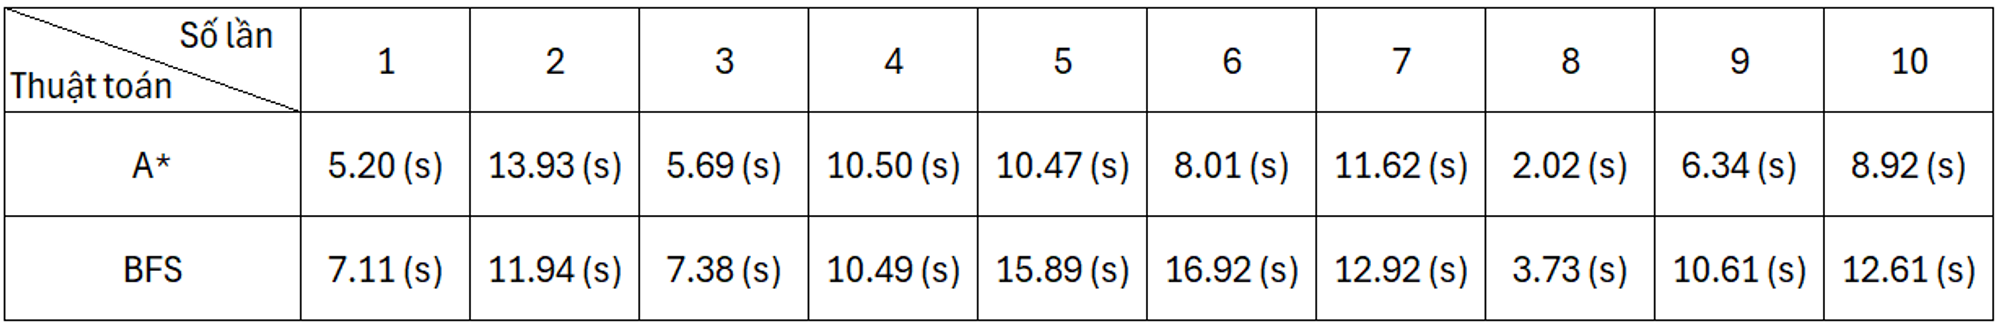
\includegraphics[width=1\linewidth]{img/compare_astar_bfs.png}
    \caption{So sánh thời gian chạy của 2 thuật toán A* và BFS}
    \label{fig:compare_astar_bfs}
\end{figure}

\paragraph{}{Có thể thấy rằng trong đa phần trường hợp, thuật toán A* sẽ có tốc độ nhanh hơn thuật toán BFS. Giải thích cho điều này là vì khác với BFS phải tìm kiếm sang toàn bộ các nút lân cận có cùng độ sâu, thuật toán A* sẽ chỉ ưu tiên tìm kiếm các nút được cho là gần hơn với mục tiêu dựa vào hàm heuristic. Vì vậy, thuật toán A* trong đa phần trường hợp sẽ duyệt qua ít đỉnh hơn so với BFS như \hyperref[fig:compare2_astar_bfs]{hình 9} (ô bắt đầu là ô màu đỏ và ô kết thúc là ô màu xanh). Mặc dù phải duyệt qua ít đỉnh hơn song thuật toán A* vẫn sẽ có trường hợp chạy chậm hơn. Đó là bởi A* sử dụng một hàng đợi ưu tiên (priority queue) có độ phức tạp khi thêm và bớt một phần tử là $O(log(n))$ với $n$ là kích thước của hàng đợi. Trong khi đó, BFS sử dụng một hàng đợi (queue) có độ phức tạp khi thêm và bớt một phần tử là $O(1)$.}

\begin{figure}[H]
    \centering
    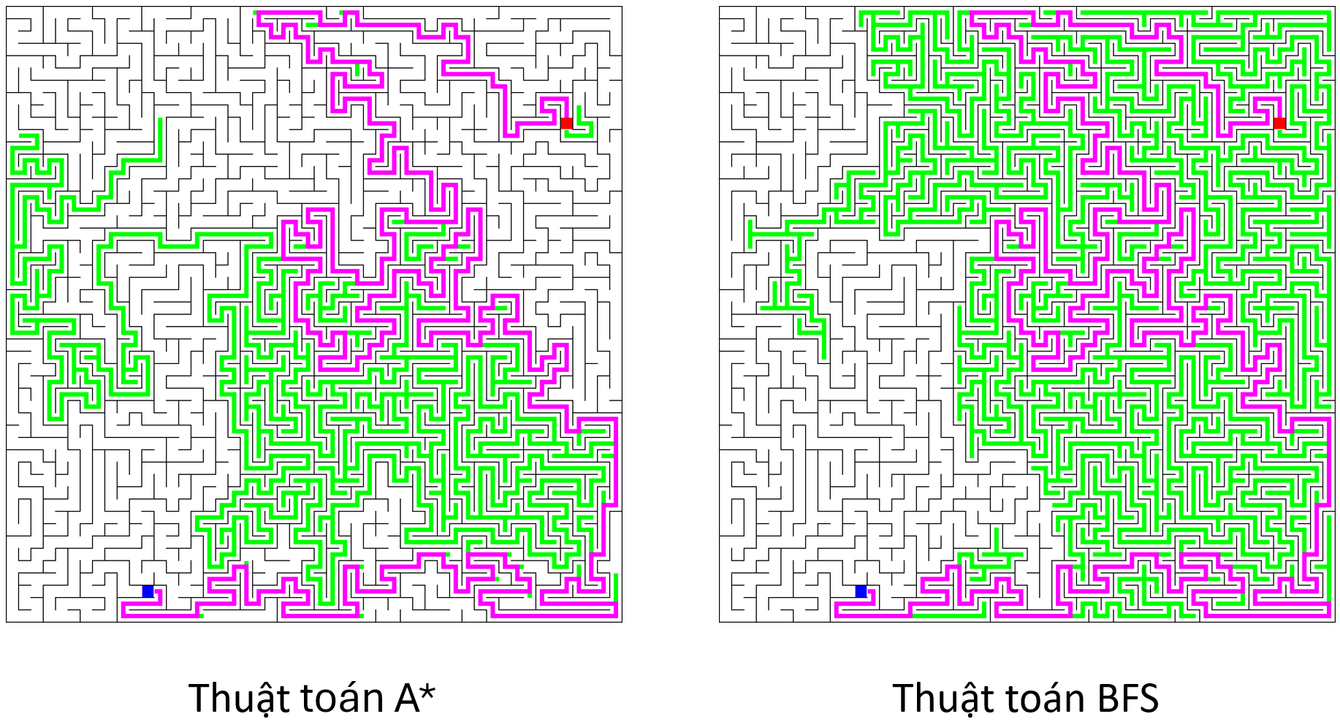
\includegraphics[width=1\linewidth]{img/compare2_astar_bfs.png}
    \caption{Minh hoạ A* và BFS tìm đường trong mê cung}
    \label{fig:compare2_astar_bfs}
\end{figure}

\paragraph{Về bộ nhớ}
\paragraph{}{Cả BFS và A* đều có độ phức tạp về không gian trong trường hợp tệ nhất là $O(|V|)$ với $|V|$ là số nút trong đồ thị. Tùy vào trường hợp đồ thị phức tạp hay không, bộ nhớ sử dụng của BFS sẽ phụ thuộc vào số nút được lưu giữ vào hàng đợi (queue). Còn đối với thuật toán A* sẽ là phụ thuộc vào hàm heuristic và số nút được đưa vào hàng đợi ưu tiên (priority queue).}


\subsection{Hệ thống gợi ý đường đi}

\paragraph{}{Để tạo hệ thống gợi ý, ban đầu sau khi sinh ra một mê cung, chúng tôi đồng thời sử dụng thuật toán BFS để xây dựng một đồ thị mới, bắt đầu duyệt từ ô kết thúc và đi tới tất cả các ô khác trong mê cung. Lúc này, đồ thị nhận được là một cây có nút gốc tương ứng với ô kết thúc của mê cung. Và vì đồ thị là một cây nên tại một nút $(x, y)$ bất kỳ, ta biết rằng nút này có duy nhất một nút cha $(u, v)$. Hướng đi từ  ô$(x, y)$ tới ô $(u, v)$ cũng là hướng đi hướng tới ô kết thúc. }

\begin{figure}[H]
    \centering
    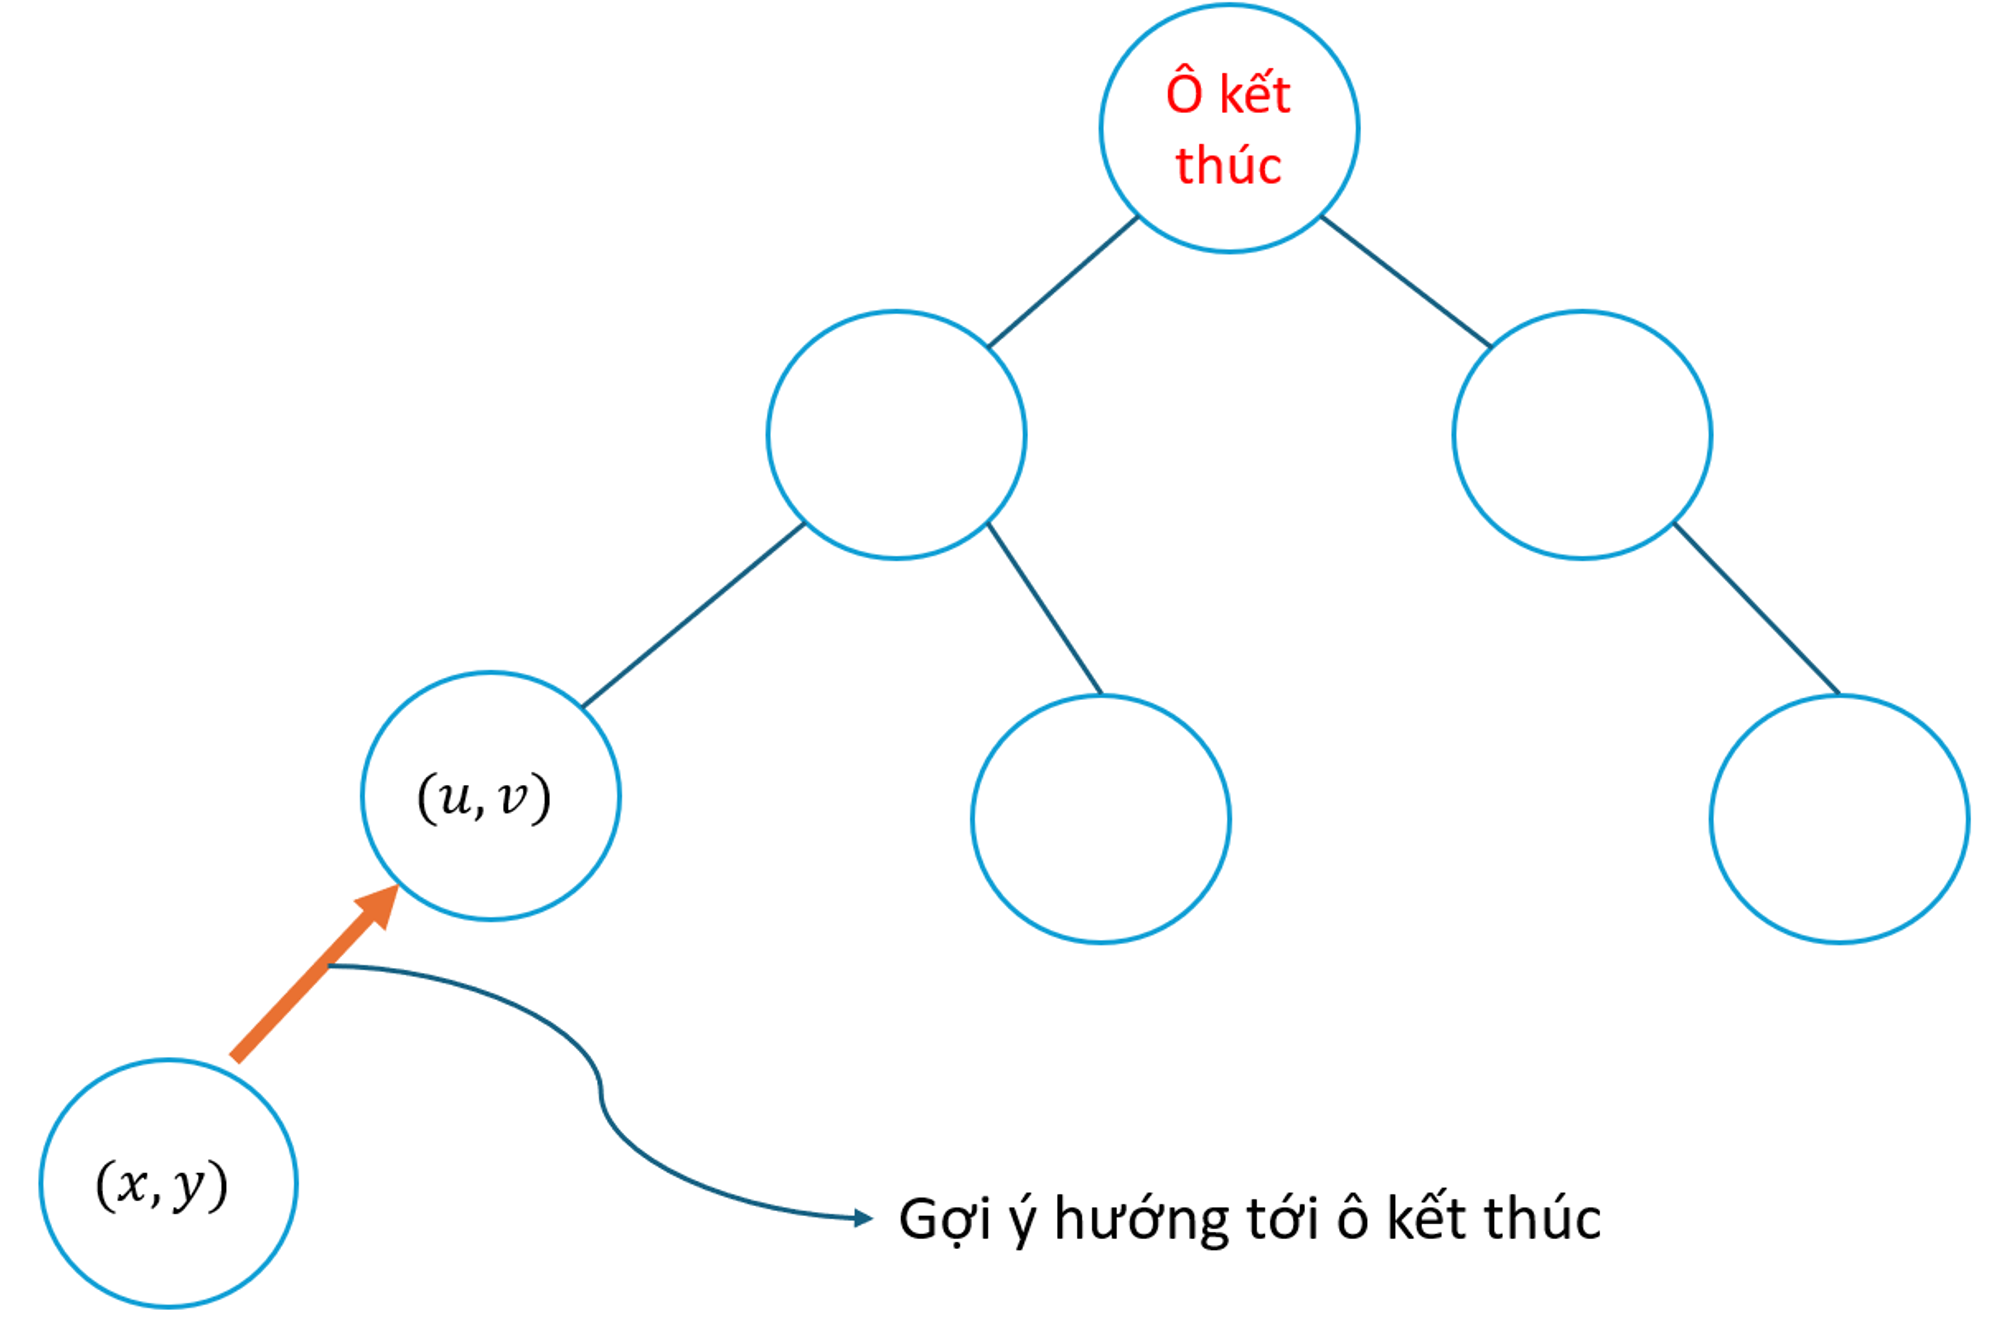
\includegraphics[width=0.7\linewidth]{img/hint_line_1.png}
    \caption{Sơ đồ cây gợi ý}
    \label{fig:hint_line_1}
\end{figure}

\paragraph{}{Sau khi người chơi ấn nút gợi ý, hệ thống sẽ tự động đưa người chơi đi theo con đường duy nhất hướng tới ô kết thúc cho đến khi gặp một ngã ba hoặc ngã tư. Lúc này, người chơi sẽ có thể tiếp tục tự mình chơi tiếp hoặc có thể ấn nút gợi ý một lần nữa.}

\begin{figure}[H]
    \centering
    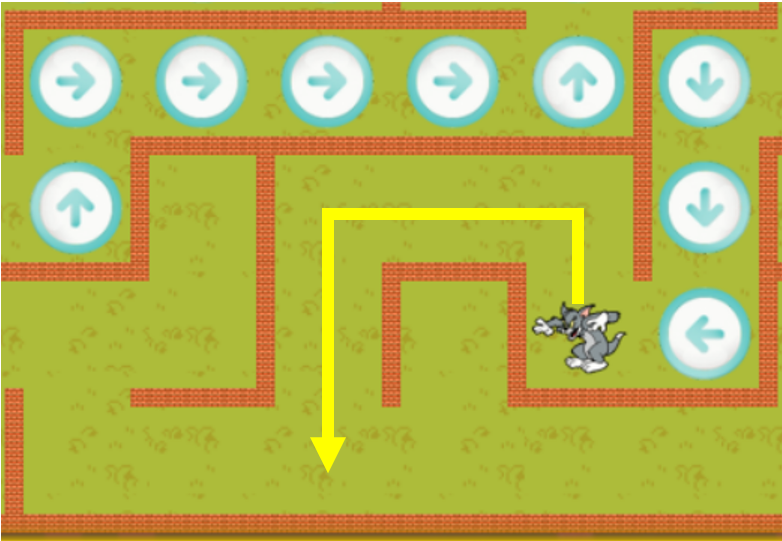
\includegraphics[width=0.7\linewidth]{img/hint_line_2.png}
    \caption{Hệ thống sẽ dẫn người chơi đi theo đường màu vàng và dừng ở ngã ba tại đầu mũi tên.}
    \label{fig:hint_line_2}
\end{figure}